\documentclass{article}
\usepackage{nips15submit_e,times}
\usepackage{graphicx} %For figure
\usepackage{caption}
\usepackage{subcaption}
\usepackage{multirow}
\graphicspath{ {./pic/} }

\title{Distributed Chat System}
\author{
Weiyao Meng\\
\And
Shuhan Wang\\
\And
Zhiyi Fan\\
\And
Junchao Wang\\
\And
Heyang Xu\\
\And
Kaimin He\\
}

\begin{document}

\maketitle

\section{Introduction}
This project is a real-time distributed chat system called HiChat that is designed as a development platform based on Java design and implementation to provide secure, efficient, easy-to-use and scalable chatroom service. This chat system sets up a Client/Server model and implements a server and multiple clients one-to-many model by forming socket network connection through TCP/IP protocol.
\\


The overall system is divided into two modules: the client and server-side functional modules. Firstly, the client is divided into user registration, registered user login, searching and adding friends, viewing the user's friends information, as well as sending and receiving texting message and image files, six service modules. HiChat application is available on Android smartphones, and for people who hate installing things, there is also a desktop application. Secondly, the server is implemented on a website which is mainly used to process the information acquire from the clients and monitor clients activities. It is divided into three service modules, the real-time monitoring, receiving and transferring a message between clients, as well as a database for storage of chatting history and user information.
\\


\section{Project Specifications}

\subsection{Desktop Application}
For the desktop application of client, firstly, a user interface is designed for users to login into this chat system according to their unique username and password. In the process, some optimizations such like the processing of incorrect characters and forgotten password will be thought. In addition, users can also register the new account in this interface which will be stored in our database automatically. When users login into the chat system successfully, the interface transfers to a chat interface. In there, users can find their friends, search the chatting records and modify some information. For the most important thing to a client, users can send messages to people who they want to chat. TCP/IP protocol is needed to establish a connection with system server so that users are able to send and receive the messages. \cite{bib2}This process is mainly achieved by JAVA Socket.\\

\subsection{Android Application}

The client is realised by Android application. In this application, there are some basic functions. 
\begin{itemize}
\item[-] The users can register an account by email. And after finishing registering, users can log in to the main chatting interface.
\item[-] The users can search their friends and add their friends in their personal contact list.
\item[-] This application can allow users chat with others by transferring text and pictures. And it also have notification function which is informing users when other users sent a message.
\item[-] This application can reserve the content of chatting with others. Moreover, the chatting content can be sent to the server and be saved on the cloud storage.
\item[-] This application can play the video format file.
\end{itemize} 
This Android application is coded by the software Android Studio or Eclipse. It can be divided into two parts that design interface and function realization. The basic Android user interface is designed by the language XML. The code of functions in Android can be set into a file called "activity".\cite{bib4} Android coding software also supports database which can be used to store the chatting content and friend contact list. Moreover, connecting to the server is achieved by HTTPS protocol which needs to establish a setup environment JDK.\cite{bib1} 


\subsection{Server Description}

The database is a software process that runs on a physical machine. Through the database process, users can manage N data space (similar to the folder) which are used to store all kinds of data (files). The process of storing data requires checking the "boundaries" where the business is planning.The information about the user account and the chat history are generally stored in a library that is mainly used when users log on to the query in the software. Each time a user logs in the system, the record of the process will be fed back to the library. In general, a service corresponds to a real database server. Sometimes in a high-end machine, it may run three service library. The software design will be based on the database load adjustment architecture. The number of accounts that can be added in the APP is limited, and the information is not written as real-time data into the database. Usually, the information will be stored in the cache and will be written into the database every few minutes to keep the database under less pressure. Otherwise, load balancing will be implemented to improve the logical server data processing and so on.

Protocols should be considered in two directions, one is about transport layer, and the other is about application layer. On the one hand, to manage the system expediently, clients are not able to directly connect with others, instead, they must depend on the server to retransmit messages and files. Thus, the chat system needs a protocol in transport layer to guarantee the connection and data exchange between server and clients. To ensure the connection is established successfully between client and server, TCP should be used in both the process of logging into the chat system, i.e., a certain client trying to establish a connection to the server and the process of transmitting messages and files.The TCP/IP protocol suite allows computers of all sizes, from many different computer vendors, running totally different operating systems, to communicate with each other.\cite{bib5}On the other hand, some protocols should be proposed in the application layer to achieve different functions of the chat system as well. The server should have the capability to analyze and classify different kinds of data received from the client to make a decision how these data will be sent to another client. Some markers should be inserted into data to let the server know whether the type of data is normal messages or files, who sent these data, and to whom these data will be sent. Also, the server needs some special protocols to invoke the database to respond requests from the client such as logging in, changing passwords, retrieving chat histories, etc. 

On the Internet, File Transfer Protocol(FTP) is needed for the two-way transmission. FTP is an application implemented in a client-server system. The client is connected to the FTP server program on the remote host through a support an FTP program, connect to the FTP server program on the remote host. After the client issues a command to the server, the server will perform commands from the client and send the results back to the client. To build a network, a pair of port socket communication providing TCP/IP encapsulation is needed, while TCP/IP provides socket interface. Socket provide IP address and port, and it builds communication between clients. Generally, each host runs multiple service software and offers several services which will open a socket and bind to a port on a different port corresponding to different services.\cite{bib3}



\section{Task Distribution}

\begin{table}

\renewcommand\arraystretch{1.5}
\newcommand{\tabincell}[2]{\begin{tabular}{@{}#1@{}}#2\end{tabular}}
\begin{tabular}{|c|c|c|p{12mm}|c|}

\hline
Number & Objectives(O) & Key Results(KRs) & \centering KR Weights & \tabincell{c}{Objectives\\Grades} \\

\hline
\multirow{2}{*}{1} & \multirow{2}{*}{\centering\parbox{1.1in}{\centering Client--Desktop\\ Application\\Student:Zhiyi Fan\\Weiyao Meng}} &\tabincell{c}{Design and implement the\\user interface for client} &\centering{50\%} &{}\\

\cline{3-5} & {} & \centering{\tabincell{c}{Design the codes of client\\Socket in order to establish\\ connection with server}}& \centering{50\%} & {} \\

\hline

\multirow{4}{*}{} & \multirow{4}*{} &\tabincell{c}{UI design of Android app} &\centering{10\%} &{}\\

\cline{3-5}{} & {} & \tabincell{c}{Research the resource of\\Android or other similar\\type chatting system} & \centering{10\%} & {} \\
\cline{3-5}{2} & {\centering\parbox{1.1in}{\centering Client--Android\\ Application\\Student:Shuhan Wang\\Kaimin He}} & \tabincell{c}{The design of basic\\function of communication\\with server and other\\ client application} & \centering{40\%} & {} \\
\cline{3-5} & {} & \tabincell{c}{The realisation of\\those basic communication\\functions and using\\socket connection to server} & \centering{40\%} & {} \\
\hline

\multirow{2}{*}{} & \multirow{3}{*}{} &\tabincell{c}{Design a wesite or a\\program for the interface.\\Implement the function of\\connections between server\\ and clients} &\centering{40\%} &{}\\
\cline{3-5}{3} & \centering\parbox{1.1in}{\centering Server\\Student:Junchao Wang\\Heyang Xu} & \tabincell{c}{Build up local database\\of file folders to\\reserve information of\\users and chat records} & \centering{30\%} & {} \\
\cline{3-5} & {} & \tabincell{c}{Extend the functions of\\the chat system and\\implement tests of program} & \centering{30\%} & {} \\
\hline

\multirow{2}{*}{4} & \multirow{2}{*}{\centering\parbox{1.1in}{\centering Final tests and\\market feasibility\\Student:All members}} & \tabincell{c}{The test of this chat\\ system, including Alpha\\test and Beta test} &\centering{80\%} &{}\\

\cline{3-5} & {} & \tabincell{c}{Expanding other functions\\of these applications and\\investigate market feasibility} & \centering{20\%} & {} \\

\hline

\end{tabular}
\caption{Tasks Allocation}
\end{table}



\newpage

\begin{figure}[h]
\centering
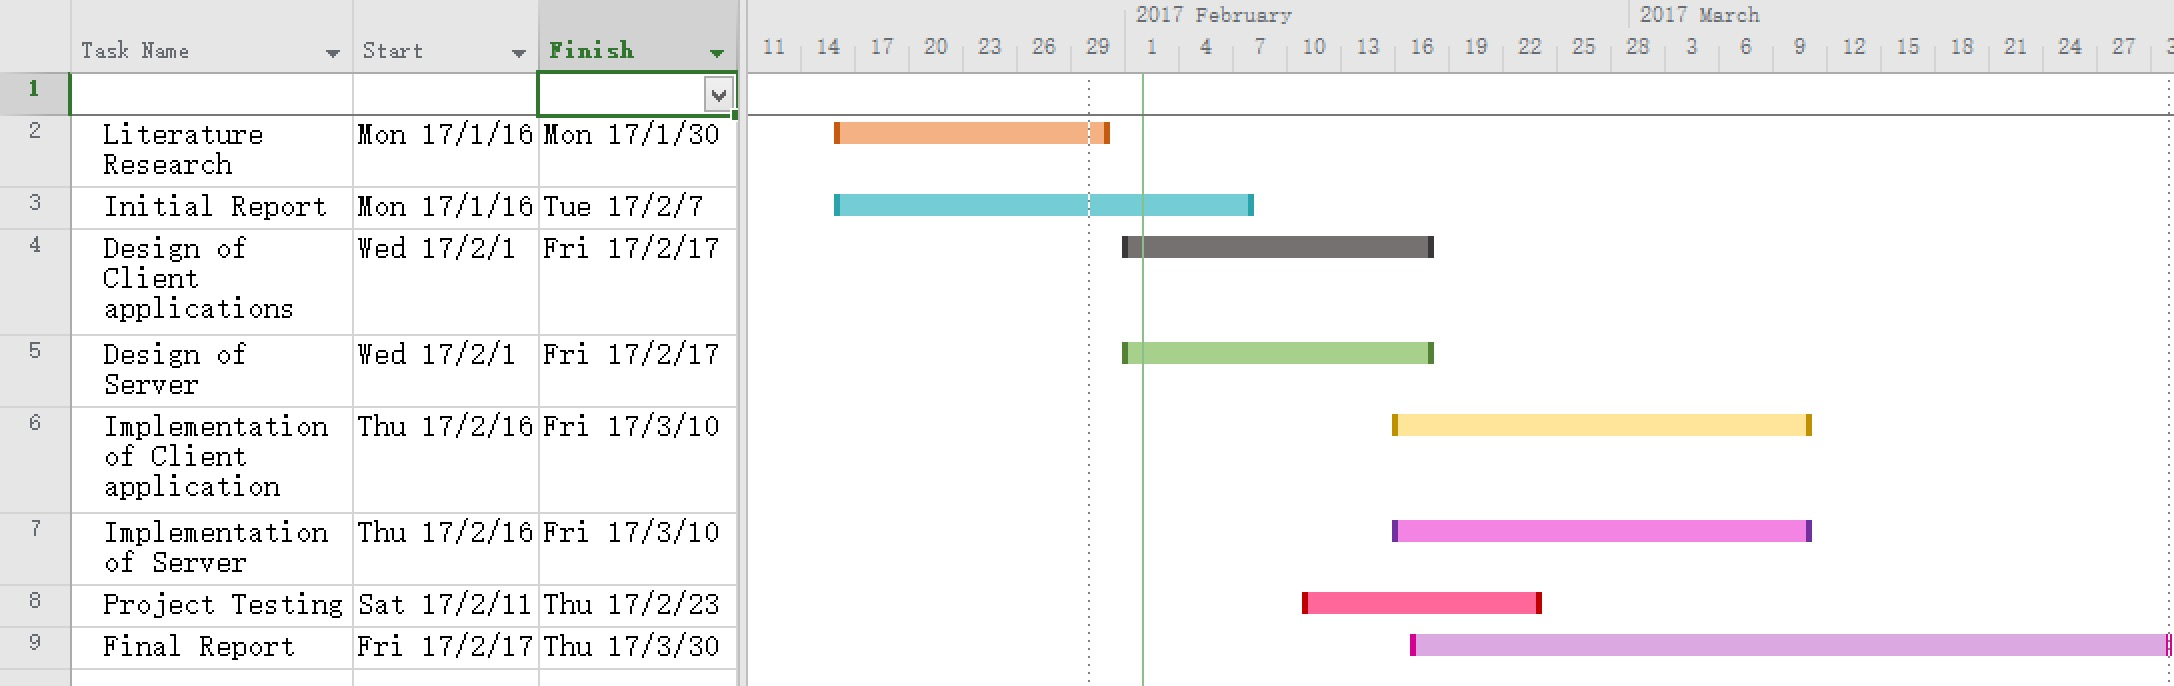
\includegraphics[width=0.7 \textwidth]{timetable.jpg}
\caption{Timetable}
\end{figure}

\section{Conclusion}

In conclusion, the aim of this project is to design a real-time distributed chat system with several functions. A server and two clients deployed in different environments will be designed and implemented. One client is a desktop application which provides a user interface, and the other one is an Android application. Particularly, TCP protocol is used to establish connections between server and clients where Socket communication is used to transmit messages. In addition, all messages will be stored in the database so that users can search the chat records and conduct more operations. Different group members are distributed to different tasks which can be seen above from Part 3 Tasks Allocation.More detailed functions of the system will be improved with the cooperation of members.




\begin{thebibliography}{9}
\bibitem{bib1} 
Darcey, L., Conder, S. \& Delessio, C. (2013). 
\textit{Sams teach yourself Android application development in 24 hours}. 
2nd edn. Indianapolis, IN: Sams Publishing.
 
\bibitem{bib2} 
Deitel, P.J. \& Deitel, H.M. (2004) 
\textit{Java how to program (6th edition) (how to program (Deitel))}. 
6th edn. Harlow, United Kingdom: Prentice Hall.
 
\bibitem{bib3} 
Goodrich, M.T. \& Tamassia, R. (2010).
\textit{Data structures and algorithms in java.}
 5th edn. New York: Wiley, John \& Sons.
 
 \bibitem{bib4} 
Lee, W.-M. (2012) 
\textit{Beginning android 4 application development}. 
 United States: John Wiley.

\bibitem{bib5} 
Marx, K., Eden, Paul, C., Cole, G.D.H. \& Wolfson, M. (1972)
\textit{ Capital: Volume I, der Produktionsprozess des Kapitals}. 
New York: J M Dent \& Sons Ltd/Everyman’s Library, United Kingdom.
\end{thebibliography}



\end{document}